\chapter{Controlling program flow}
\label{chap:flow}
Non-recursive functions encapsulates code and allows for some control of flow, that is, if there is a piece of code, which we need to to have executed many times, then we can encapsulate it in the body of a function, and then call the function several times. In this chapter, we will look at more general control of flow via loops, conditional execution, and recursion, and therefore we look at further extension of the \lstinline[language=ebnf]!expr! rule,
\begin{lstlisting}[language=ebnf]
pat = const | ...
guard = "when" expr
rule = pat [guard] -> expr
rules = "|" rule | "|" rule rules (* first "|'' is optional' *)
expr = ... 
  | "for " pat " in " expr " do " expr [" done "] (* for expression *)
  | "for " var "=" expr " to " expr " do " expr [" done "] (* simple for expression *)
  | "while " expr " do " expr [" done "] (* while expression *)
  | "if " expr " then " expr {" elif " expr " then " expr} " else " expr (*  conditional expression *)
  | "match " expr " with " rules (* match expression *)
  | "function " rules (* matching function expression *)
  | "let " rec function-or-value-defns (* recursive definition *)
  | ...
\end{lstlisting}

\section{For and while loops}
Many programming constructs need to be repeated. The most basic example is counting, e.g., from 1 to 10 with a \idx{\keyword{for}}-loop,
%
\fso{count}{Counting from 1 to 10 using a \keyword{for}-loop.}
%
As this interactive script demonstrates, the identifier \lstinline!i! takes all the values between 1 and 10, but in spite of its changing state, it is not mutable. Note also that the return value of the \keyword{for} expression is \token{()} like the \lstinline!printf! functions. The \keyword{for} and \keyword{while} loops follow the syntax,
\begin{lstlisting}[language=ebnf]
pat = const | ...
expr = ... 
  | "for " pat " in " expr " do " expr [" done "] (* for expression *)
  | "for " var "=" expr " to " expr " do " expr [" done "] (* simple for expression *)
  | "while " expr " do " expr [" done "] (* while expression *)
 | ...
\end{lstlisting}
Using lightweight syntax the script block between the \keyword{do} and \keyword{done} keywords may be replaced by a newline and indentation, e.g.,
%
\fs{countLightweight}{Counting from 1 to 10 using a \keyword{for}-loop.}
%
A more complicated example is,
\begin{problem}
  Write a program that prints the $n$'th fibonacci number.
\end{problem}
The fibonnacci numbers is the series of numbers $1,1,2,3,5,8,13\dots$, where the $\text{fib}(n) = \text{fib}(n-1)+\text{fib}(n-2)$, and they are related to Golden spirals shown in Figure~\ref{fig:goldenSpiral}.
\begin{figure}
  \centering
  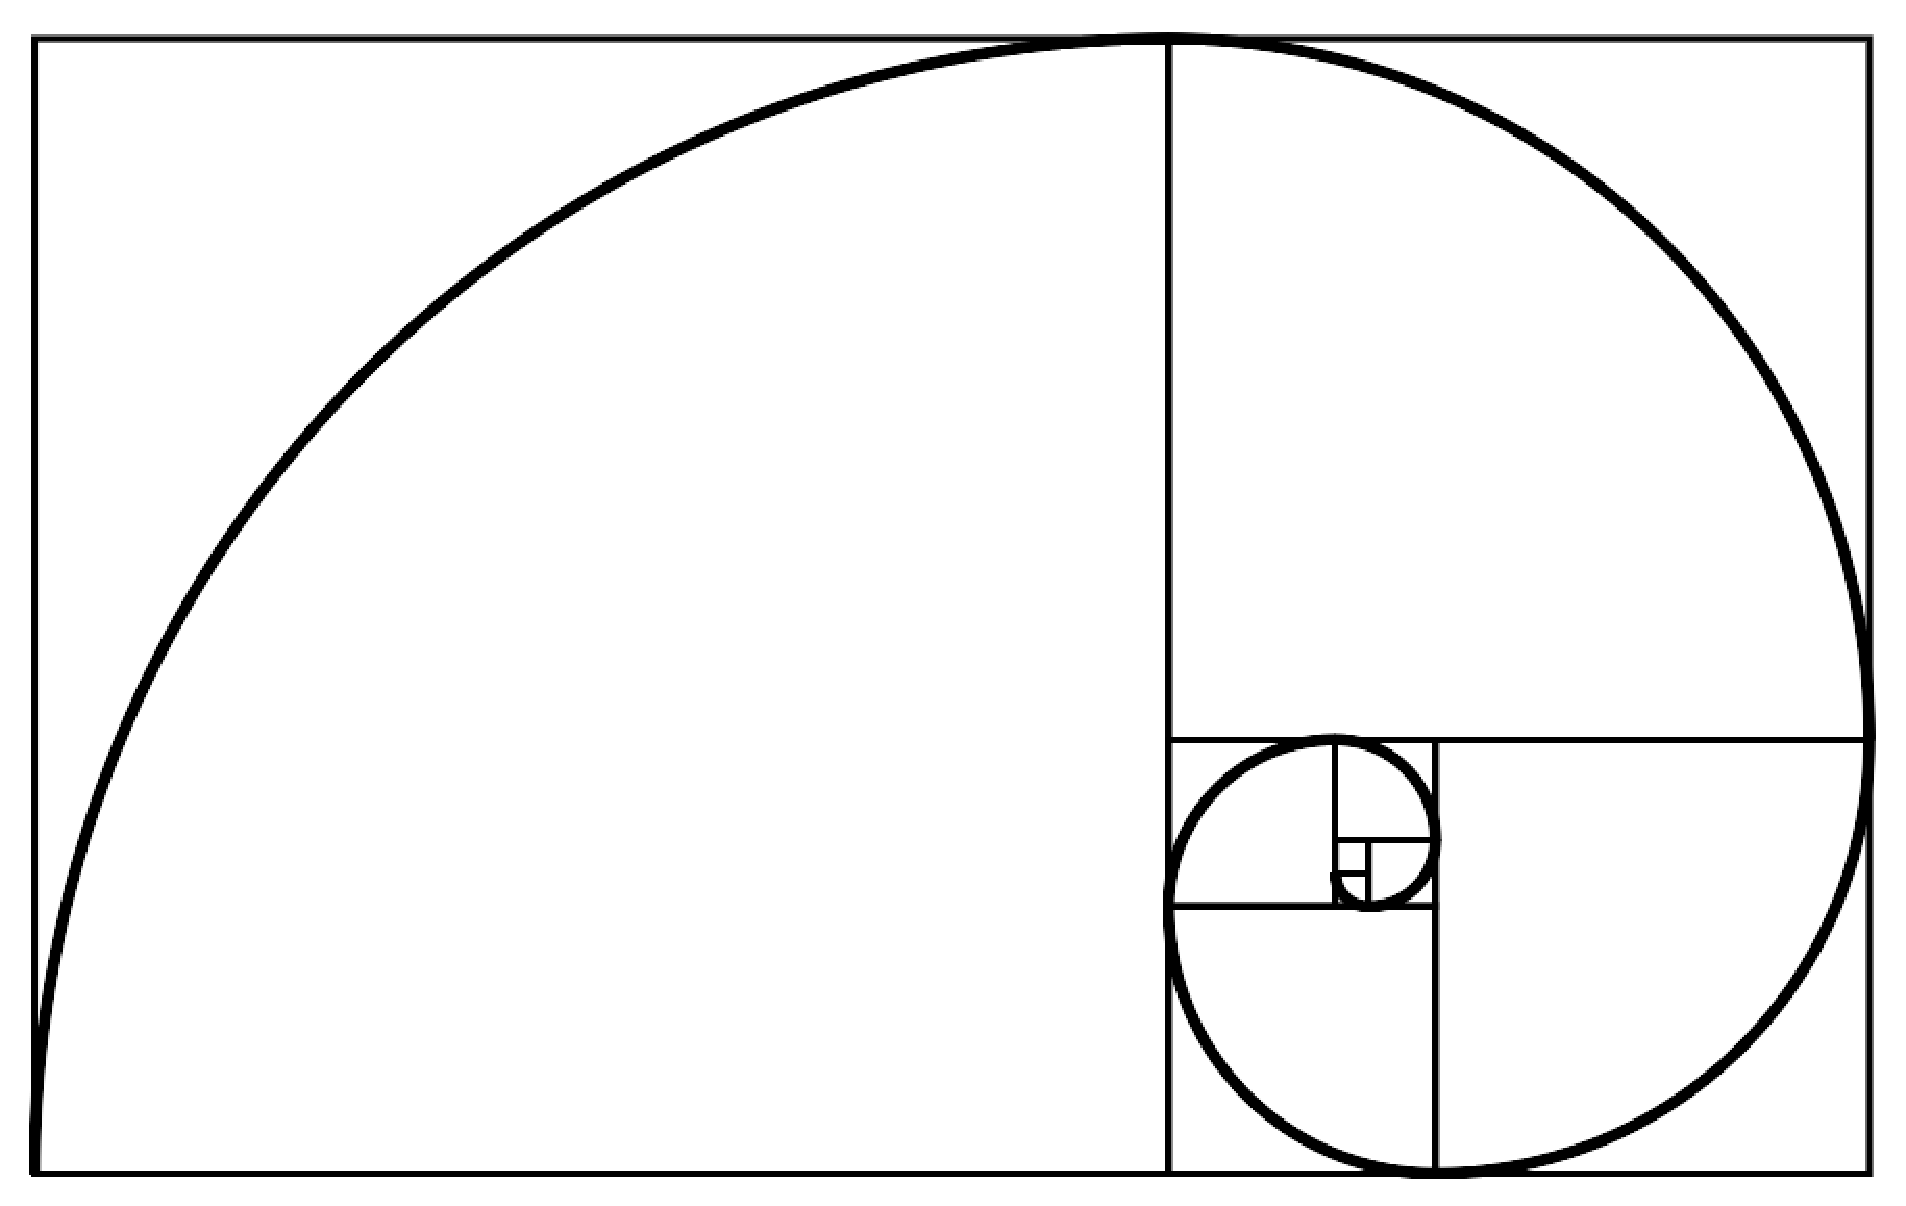
\includegraphics[width=0.45\linewidth]{Fibonacci_spiral_34}
  \caption{The fibonacci spiral is an approximation of the golden spiral. Each square has side lengths of successive fibonacci numbers, and the curve in each square is the circular arc with radius of the square it is drawn in. Figure by Dicklyon \url{https://commons.wikimedia.org/w/index.php?curid=3730979}}
  \label{fig:goldenSpiral}
\end{figure}
We could solve this problem with a \keyword{for}-loop as follows,
%
\fs{fibFor}{The $n$'th fibonacci number as the sum of the previous 2 numbers, which are sequentially updated from 3 to $n$.}
%
The basic idea of the solution is that if we are given the $(n-1)$'th and $(n-2)$'th numbers, then the $n$'th number is trivial to compute. And assume that $\text{fib}(1)$ and $\text{fib}(2)$ are given, then it is trivial to calculate the $\text{fib}(3)$. Now we have the first 3 numbers, so we disregard $\text{fib}(1)$ and calculate $\text{fib}(4)$ from $\text{fib}(2)$ and $\text{fib}(3)$, and this process continues until we have reached the desired $\text{fib}(n)$

For the alternative \keyword{for}-loop, consider the problem,
\begin{problem}
  Write a program that identifies prime factors of a given integer $n$.
\end{problem}
Prime numbers are integers divisible only be 1 and themselves with zero remainder. Let's assume that we already have identified a list of primes from 2 to $n$, then we could write a program that checks the remainder as follows,
%
\fs{primeCheck}{Checking whether a given number has remainder zero after division by some low prime numbers.}
%
In this example, the variable \lstinline!i! runs through the elements of a list, which will be discussed in further detail in Chapter~\ref{chap:lists}.

The \idx{\keyword{while}}-loop is simpler than the \keyword{for}-loop and does not contain a builtin counter structure. Hence, if we are to repeat the count-to-10 program from Listing~\ref{count} example, it would look somewhat like,
%
\fs{countWhile}{Count to 10 with a counter variable.}
%
In this case, the \keyword{for}-loop is to be prefered, since more lines of code typically means more chances of making a mistake. But the \keyword{while}-loop allows for other logical structures. E.g., lets find the biggest fibonacci number less than 100,
%
\fs{fibWhile}{Search for the largest fibonacci number less than a specified number.}
%
Thus, \keyword{while}-loops are most often used, when the number of iteration cannot easily be decided, when entering the loop.

Both \keyword{for}- and \keyword{while}-loops are often associated with variables, i.e., values that change while looping. If one mistakenly used values and rebinding, then the result would in most cases be of little use, e.g.,
%
\fs{forScopeError}{Lexical scope error. While rebinding is valid F\# syntax, has little effect due to lexical scope.}
%
I.e., the \keyword{let} expression rebinds \lstinline!a! every iteration of the loop, but the value on the right-hand-side is taken lexically from above, where \lstinline!a! has the value 1, so everytime the result is the value 2.

\section{Conditional expressions}
\begin{lstlisting}[language=ebnf]
"if" expr "then" expr 
[{"elif" expr "then" expr}
"else" expr]
\end{lstlisting}
A basic flow control mechanism used both for functional and imperative programming is the \texttt{if-then-else} construction, e.g.,
\fs{flowIfThen}{}
I.e., if and only if the value of the argument is postive, then it will be printed on screen. More common is to include the \texttt{else} 
\fs{flowIfThenElse}{}
A common construction is a nested list of \texttt{if-then-else},
\fs{flowIfThenElseNested}{}
where the integers 0--2 are converted to characters, and integers outside this domain is converted to the nearest equivalent number. This construction is so common that a short-hand notation exists, and we may equivalently have written,
\fs{flowIfThenElseNestedShort}{}

\section{Pattern matching}
Often functions are needed, that performs different calculations based on the input values. E.g., counting items in the english language requires various forms depending on the number, so we would say ``I have 1 apple'' and ``I have 2 apples''. For this we may use the \keyword{match}-\keyword{with} programming construct, and a function that given a number returns a string on propper form could look like,
%
\fs{matchWith}{Using the \keyword{match}-\keyword{with} programming construct to vary calculation based on the input value.}
%
This is an example of controlling programming flow, which will be discussed in more depth in Chapter~\ref{chap:flow}.
\begin{lstlisting}[language=ebnf]
expr = ... | "match " expr " with " rules 
rule = pat [guard] -> expr
guard = "when" expr
pat = const | ...     
\end{lstlisting}

Functions may be declared using pattern matching, which is a flexible method for declaring output depending on conditions on the input value. The most common pattern matching method is by use of the \texttt{match with} syntax,
\fs{functionDeclarationMatchWith}{}

A short-hand only for functions of 1 parameter is the \texttt{function} syntax,
\fs{functionDeclarationFunction}{}
Note that the name given in the match, here \texttt{n}, is not used in the first line, and is arbitrary at the line of pattern matchin, and may even be different on each line. For these reasons is this syntax discouraged.

\section{Recursive functions}
\jon{Recursive functions here.}

\dots
A major difference between functional and imperative programming is how loops are expressed. Consider the problem of printing the numbers 1 to 5 on the console with a \keyword{while} loop can be done as follows,
\fs{countWhile}{}
where the same result by recursion as
\fs{flowWhileRecursion}{}
The counting example is so often used that a special notation is available, the \keyword{for} loop, where the above could be implemented as
\fs{flowFor}{}
Note that \texttt{i} is a value and not a variable here. For a more complicated example, consider the problem of calculating average grades from a list of courses and grades. Using the above construction, this could be performed as,
\fs{flowForListsIndex}{}
However, an elegant alternative is available as
\fs{flowForLists}{}
This to be preferred, since we completely can ignore list boundary conditions and hence avoid out of range indexing. For comparison see a recursive implementation of the same,
\fs{flowForListsRecursive}{}
Note how this implementation avoids the use of variables in contrast to the previous examples.


%%% Local Variables:
%%% TeX-master: "fsharpNotes"
%%% End:
